\begin{figure*}
\begin{center}
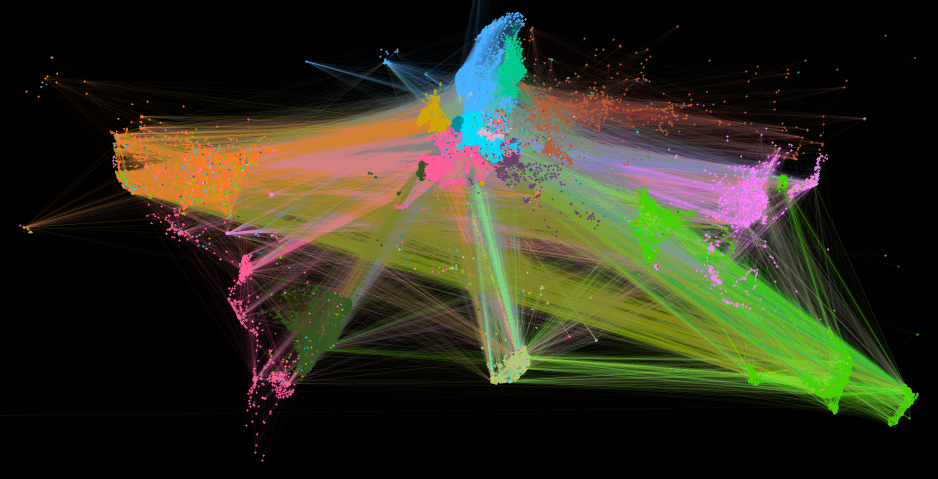
\includegraphics[width=.65\textwidth]{fig1.png}
\end{center}
\caption{Global network of interlocking directorates. Color indicates communities -- i.e. cities that do business together within each other more often than with others.}
\label{fig:fig1}
\end{figure*}

\section{Research questions, concepts and propositions}
\label{sec:question}
\subsection{Interlocking directorates}
Companies are embedded in complex networks of `interlocking directorates' -- 
created when directors from a corporation sit on multiple boards.
The relationship between two corporations resulting from a director sitting in both of their boards is often referred to as a direct interlock~\citep{Mizruchi1996} (Fig.~\ref{fig:bipartite}).
Interlocks can also be indirect when two directors from two firms sit together on the board of directors of a third firm. 
Several explanations (micro-motives) have been pointed out for the creation of interlocks. 
These include facilitating cooperation to limit competition (collusion),  
absorption of potentially disruptive elements (cooptation), 
creating legitimacy by hiring respectable directors, 
career advancement, and social cohesion~\citep{Mizruchi1996}.

\begin{figure}
\begin{center}
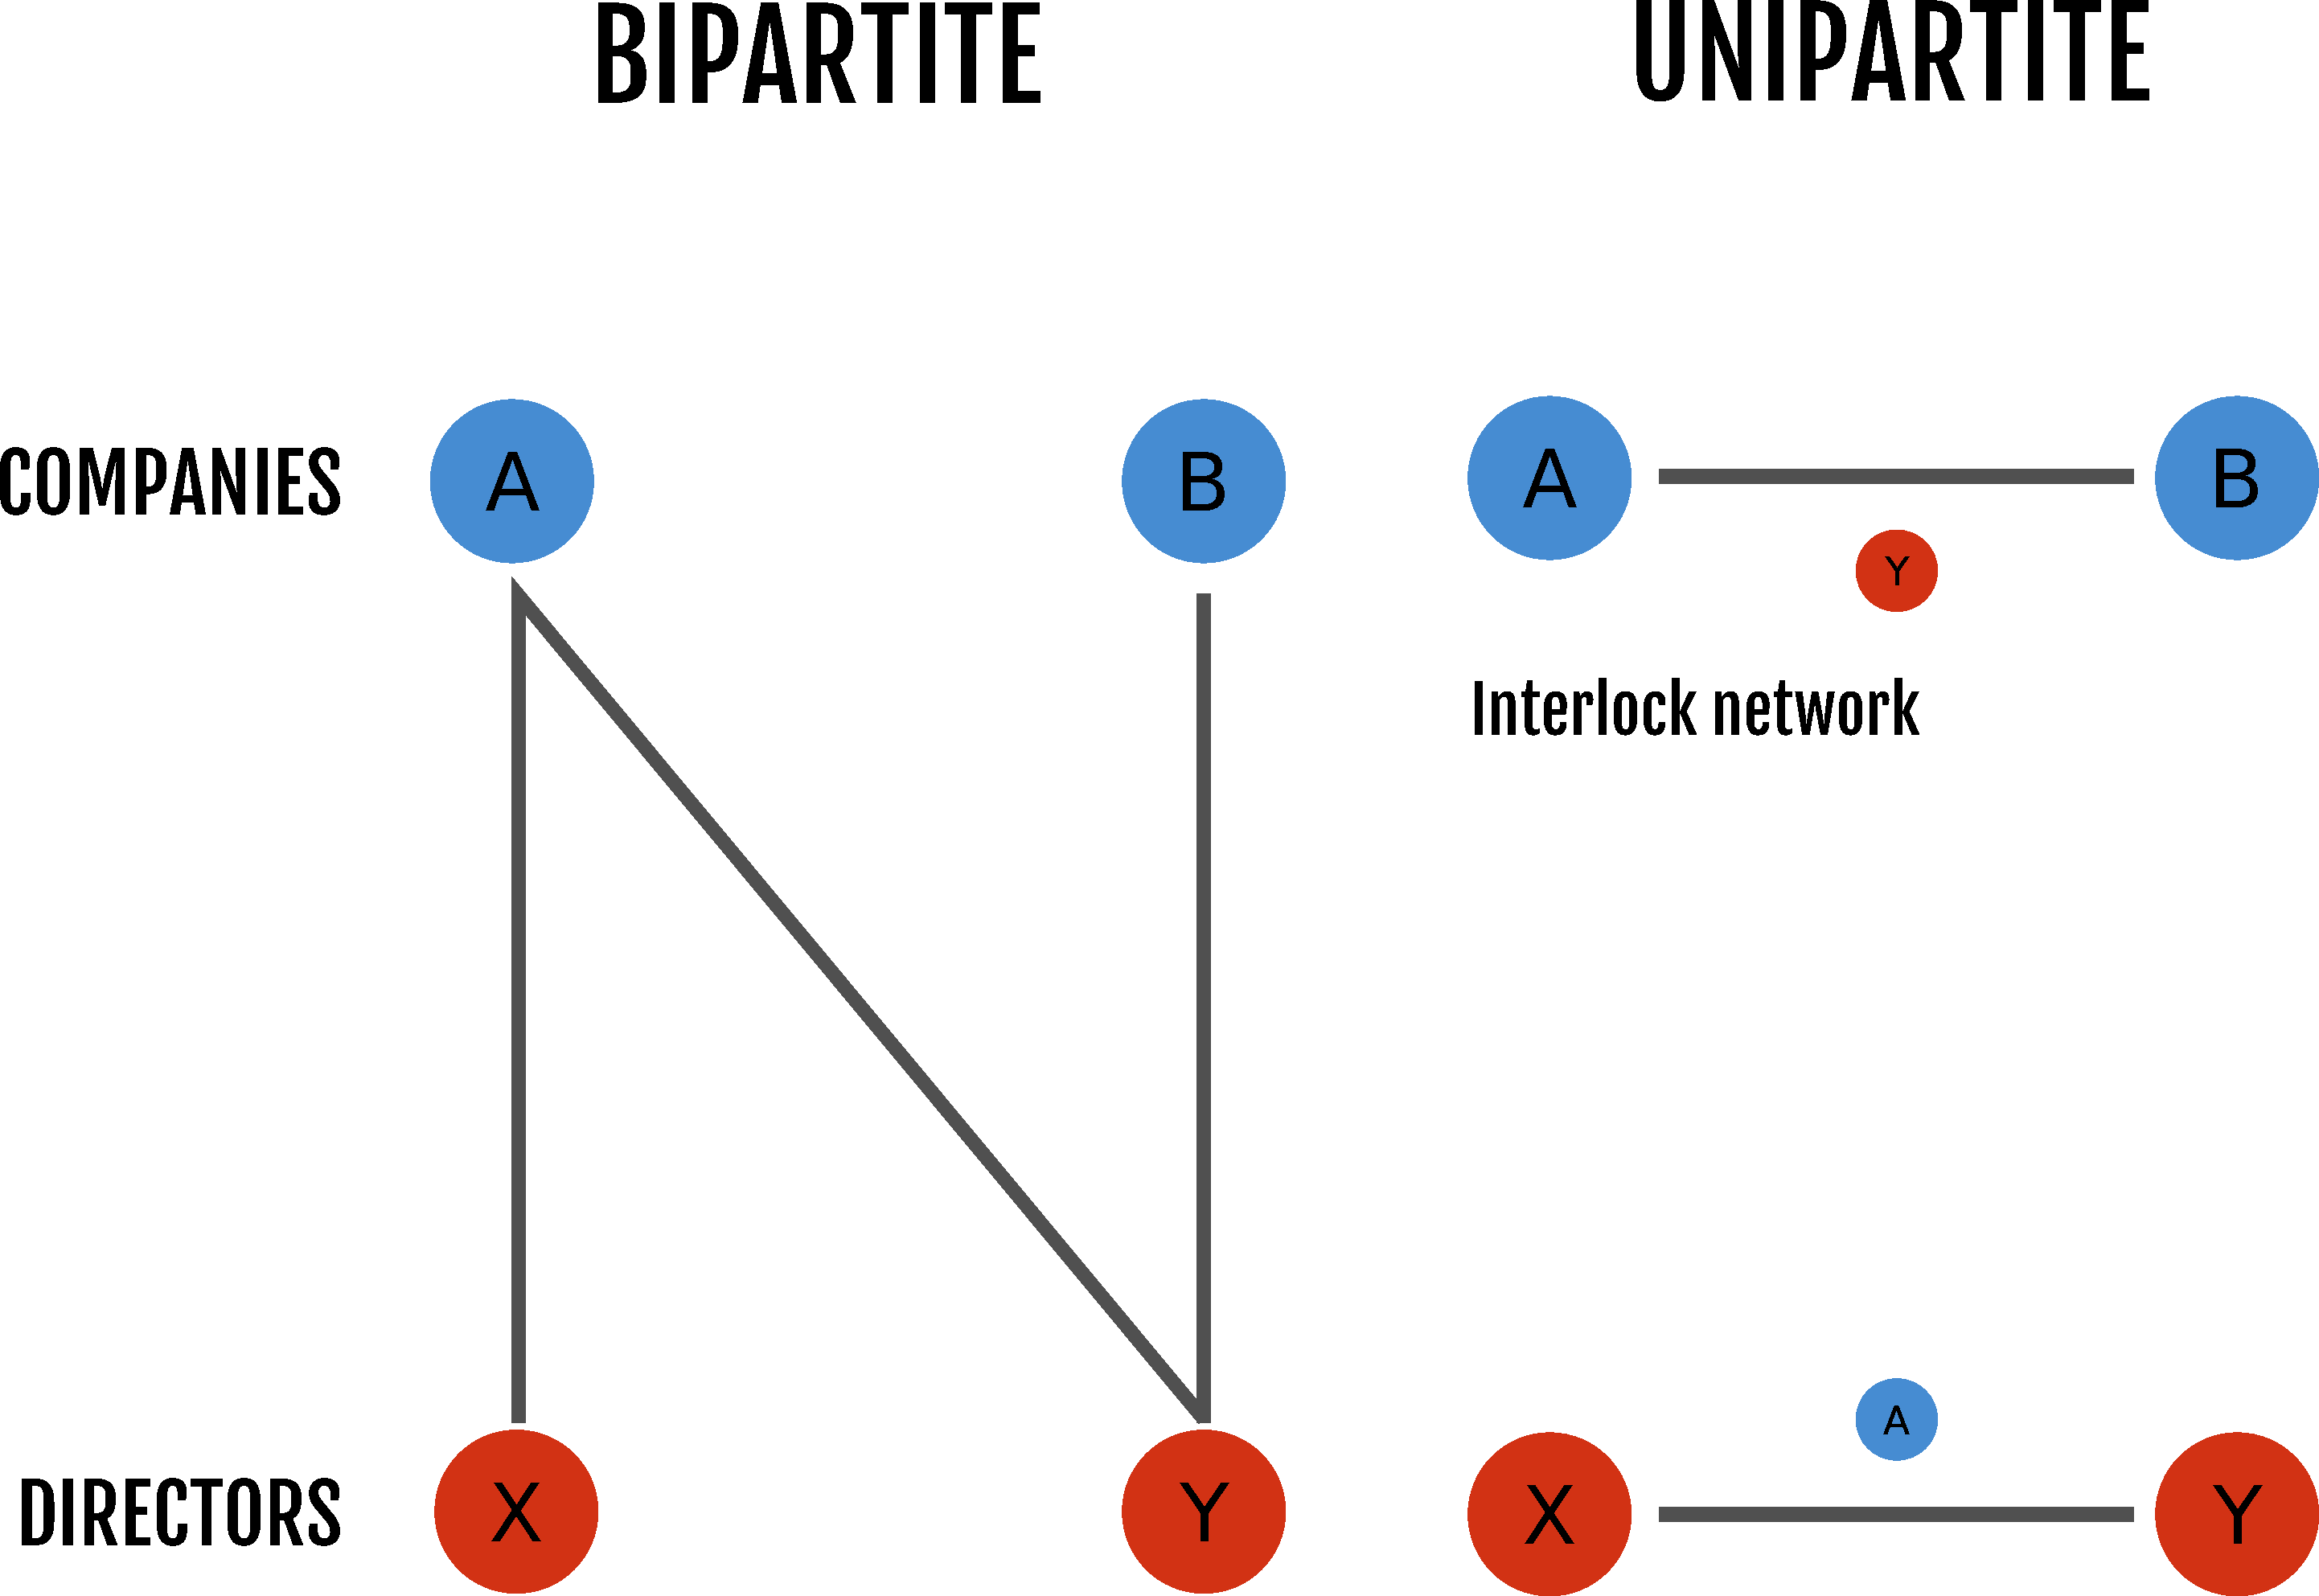
\includegraphics[width=.45\textwidth]{bipartite.pdf}
\caption{\textbf{Two-modes and one-mode networks}. Relationship between companies and directors (bipartite network) and one-mode projections (unipartite networks). Company A and B have a direct interlock}
\label{fig:bipartite}
\end{center}
\end{figure}

Although the micro-motives for the existence of interlocks are relatively well understood, 
their effects are still object to controversy. 
In the past decades, many papers have investigated the effect of interlocks in firm performance, innovation, acquisitions, mergers, capital growth, firm reputation, and the adoption of structures and strategies(see Mizruchi~\cite{Mizruchi1996} for a review).
However, only the spread of structures and strategies has been consistently associated to interlocks~\citep{Haunschild1993,Davis1997,Davis1991,Rao1999,Shropshire2010} .
We attribute this to limitations in the data and to the assumption of a linear system instead of a complex system (please see section ~\ref{sec:data} for an analysis of complex systems and their relevance in social systems).
Previous papers have focused on a small number of top companies (10--1000), 
many times restricting the study to only one sector or country. 
The result of this approach is a misrepresentation of local patterns as global patterns.
For example, 
Peng et al.~\citep{Peng2016}, using a survey of 27 managers from 20 firms in a major industrial center in Jiangsu province (China), found that the presence of interlocks increases firm growth.
At the same time,
Non and Franses~\citep{franses2007interlocking}, using annual reports from the largest 101 Dutch companies, found that the presence of interlocks decreases firm performance.
Recognizing that the system is multi-level (directors and companies) can help bring insight to this processes.
For instance, we can assume two types of ties director-firm. 
The first type is status ties.
People seek employment in companies that are rapidly growing,
while companies that are rapidly growing seek new people to continue their expansion.
The second type is monitoring ties.
Companies that invested heavily in company A will demand to place one of their own directors on A's board in order to monitor its activity.
The result of this model is an inverse U-shaped relationship between firm performance and number of interlocks.
Moreover, this model can be directly tested linking monitoring ties to interlocks with an ownership relationship between companies, 
and status ties to interlocks without ownership relationships.


% simple explanation by Mizruchi~\cite{Mizruchi1996} that 
%For instance,  points out that if directors are appointed when the productivity of the firm is low (as a form of monitoring),
%and directors decide to join boards that are performing well (as a form of career development),
%the end result would be an inverted U shaped relationship between number of interlocks and firm performance. 
%This model would explain why researchers [refs] have found positive and negative relationship between interlocks and performance,


Here, we study a large dataset comprising 200 million companies and 100 million directors (see \ref{sec:data}) to bring definitive answers to the field.
Our main research question is ``How is the network of interlocking directorates structured in time and space, and what is its effect on structural transformation?''.
For the sake of brevity, we focus here on the second part of the question ``what is the effect of interlocks on structural transformation'',
where structural transformation corresponds to the evolution of the distribution of economic activities within the city.
In section \ref{sec:pss} we explore the concepts of structural transformation and the product-service space.
The product-service space determines how closely two economic activities (sectors) are depending on how often companies from both sectors are co-located in the same city.
In section \ref{sec:interlockspss}, we determine if (and how) interlocks affect structural transformation.
Section \ref{sec:factors} shows what factors influence the presence of interlocks.
Our unit of analysis can be the company itself, the city, the country or the region. 
Although the analysis will be done at multiple scales,
we will focus on the city level for the rest of the manuscript.
The focus at the city level allows us to link our research to both the existing literature on cities as engines of technological growth (see for example ~\citep{Belderbos2014}),
and to existing databases on human and economic capital.


\subsection{Product-service space}
\label{sec:pss}
Cities and countries develop economically by moving from producing simple products and services to specializing in more expensive ones -- a process referred to as `structural transformation'~\citep{smith1776, Romer1991,grossman1991,hidalgo2007}.
This transformation can be explained using differences in productive factors and technology (see~\citep{hausmann2011} for a review).
In order to connect these differences to development, 
current models usually abstract from the products and look at macro-indicators of productive factors and technology.
However, development occurs when new products are created or existing ones improved,
and it is not clear if these models can explain the variability observed in countries with similar macro-indicators.
Moreover, the products that are developed depend on the current products being produced -- there is a relatedness between products.
Many explanation have been proposed for this, 
such as similar institutions, infrastructure, physical factors, technology, or some combination of those factors (see~\cite{hidalgo2007} for a review).
To reconcile previous research without abstracting from the products,
Hidalgo, Hausmann and Klinger~\cite{hidalgo2007, hausmann2011, Hausmann2006,hidalgo2009} assumed that related products require similar underlying factors (`capabilities').
They next developed the `product space' as a map of the relatedness between products,
where products are related if countries have competitive advantages respect to both products.
They showed that the product space capture information about the set of capabilities available in a country, 
is strongly correlated with income per capita, 
and predictive of future growth.
Furthermore, they proved that structural transformation at the country level occurs by moving from existing products to related products, 
where two products are related if they are close in the `product space'.

In a world full of multi-national companies, innovation is happening at the city level~\citep{Belderbos2014}.
To account for an exploration of the process at the city-level, we need adapt the `product-space' concept. 
We will create the `product-space' using relationships between economic activities at the city level, weightining economic activities by revenue per employee (since value added is not available for more than 1\% of the companies),
instead of using product categories at the country level as in~\cite{hidalgo2007, hausmann2011, Hausmann2006,hidalgo2009}.
Using cities allows us to explore not only products, but also services, thus we will define the `product-service space'. 
The subquestion here is: ``Does structural transformation at the city follows the links of the product-service space''.
We expect to find comparable trends at the city level to those found by Hidalgo, Hausman and Klinger at the country level.
The structural transformation should follow the edges in the product-service space, 
and the diffusion process should correlate with gdp per capita in the city (the OECD database provide city-level data), 
and maybe with innovation, for which we can use the city Innovation index \footnote{\url{http://www.innovation-cities.com/innovation-cities-index-2015-global/9609}}
or the number of patents developed in companies from the city.
The causal argument is symmetrical from Hidalgo, Hausman and Klinger's argument~\cite{hidalgo2007, hausmann2011, Hausmann2006,hidalgo2009} but at the city level.
Cities require some underlying capabilities (infrastructure, education, institutions, human capital) to maintain specific companies,
and those capabilities are similar for economic activities close together in the product-service space.
When a city acquire new capabilities, new products can be developed along the product-service space.
Since we are more interesting in understanding the role of interlocks in the process, 
the aim of this section is descriptive, 
but hinting on causality.
Negative results would suggest an extreme globalization of the cities, 
where the benefit of having `in situ' capabilities is minimal.
Importantly, we expect to see differences accross space and time.
The study of these differences would allow us to link diffusion patterns to varieties in capitalism, 
and analyze if liberal market economies (e.g., U.S., U.K.) and coordinated market economies (e.g. Germany, France) are converging.

%We will define the network as $PSS = (V, E)) $, where $V$ are the sectors according to NACE rev. 2 (e.g. C11 = Manufacture of beverages),
%and $E$ is the matrix of weights between sectors.


\subsection{Interlocks and the product-service space}
\label{sec:interlockspss}
%[Research subquestion herere]
Next, we will analyze if interlocks are a good predictor of diffusion between economic activities in cities. 
Development itself influences the presence of interlocks.
Companies situated close geographically, or in places with similar language or colonial ties 
have greater chances to interlock~\citep{nobel2004economische}.
Since the establishment of companies within a city allows for greater possibilities of interlocks,
we expect a relationship between the product-service space and the number of interlocks between economic activities.
However it is not clear if interlocks are only a cause of development but also an effect.
Interlocks provide a communication channel between companies, 
and serve as a link for the spread of strategies and structures.
For instance, acquisition behaviours in one company are imitated by companies linked by interlocks~\citep{Haunschild1993}.
The spread of poison pills (securities that give target shareholders the right to buy shares at a 50\% discount in the case of hostile takeovers) increased from 5\% to 35\% adoption in 1987 through interlock and ownership links~\cite{Davis1997,Davis1991}. 
Similarly, companies linked by interlocks move together to new stock markets~\citep{Rao1999}.
We hypothesize that interlocks serve as a communication channel between companies,
which allows for the spread of business opportunity and collaboration,
thus increasing investment and R\&D fund to promising sectors (those close in the product-service space).
Moreover, increased investment and innovation has been linked to economic development~\citep{Romer1991,grossman1991,hidalgo2007}.
In a first step, we will test if interlocks affect the diffusion process in the product-service space,
and how netwrok characteristics affect city outcomes.
In a second step, we will analyze collaboration between companies using patent data to show if this diffusion process is mediated (at least partially) by innovation.

\subsubsection{Interlocks affect the product-service space}
%[Research subquestion herere]
Figure ~\ref{fig:entropy} shows our approach. 
Given the number of companies in city A at time $t$ (Fig. ~\ref{fig:entropy}A), 
we want to explain the evolution to time $t+1$ (Fig. ~\ref{fig:entropy}B).
This evolution occur in the edges of the `product space' (Fig. ~\ref{fig:entropy}C).
We can create a network of interlocks (Fig. ~\ref{fig:entropy}D),
where two economic activities are connected if a director sits in companies from both sectors.
Importantly, the network of interlocks have relationships between sectors that are not present in Figure ~\ref{fig:entropy}A. 
This is because interlocks are not restricted to the city itself.
A director can sit in the banking sector in city A and in the IT sector in city B, even if there are no IT companies in city A.
Our research question here is ``To what extent do interlocks increase the diffusion rates in the product-service space?''.
As explained in the previous section, 
we expect people to spread ideas and information among the boards where they sit on.
Thus, interlocks serve as a communication channel between companies, 
which in turn would increase investment and R\&D fund to promising sectors (those close in the product-service space).

\begin{figure}
\begin{center}
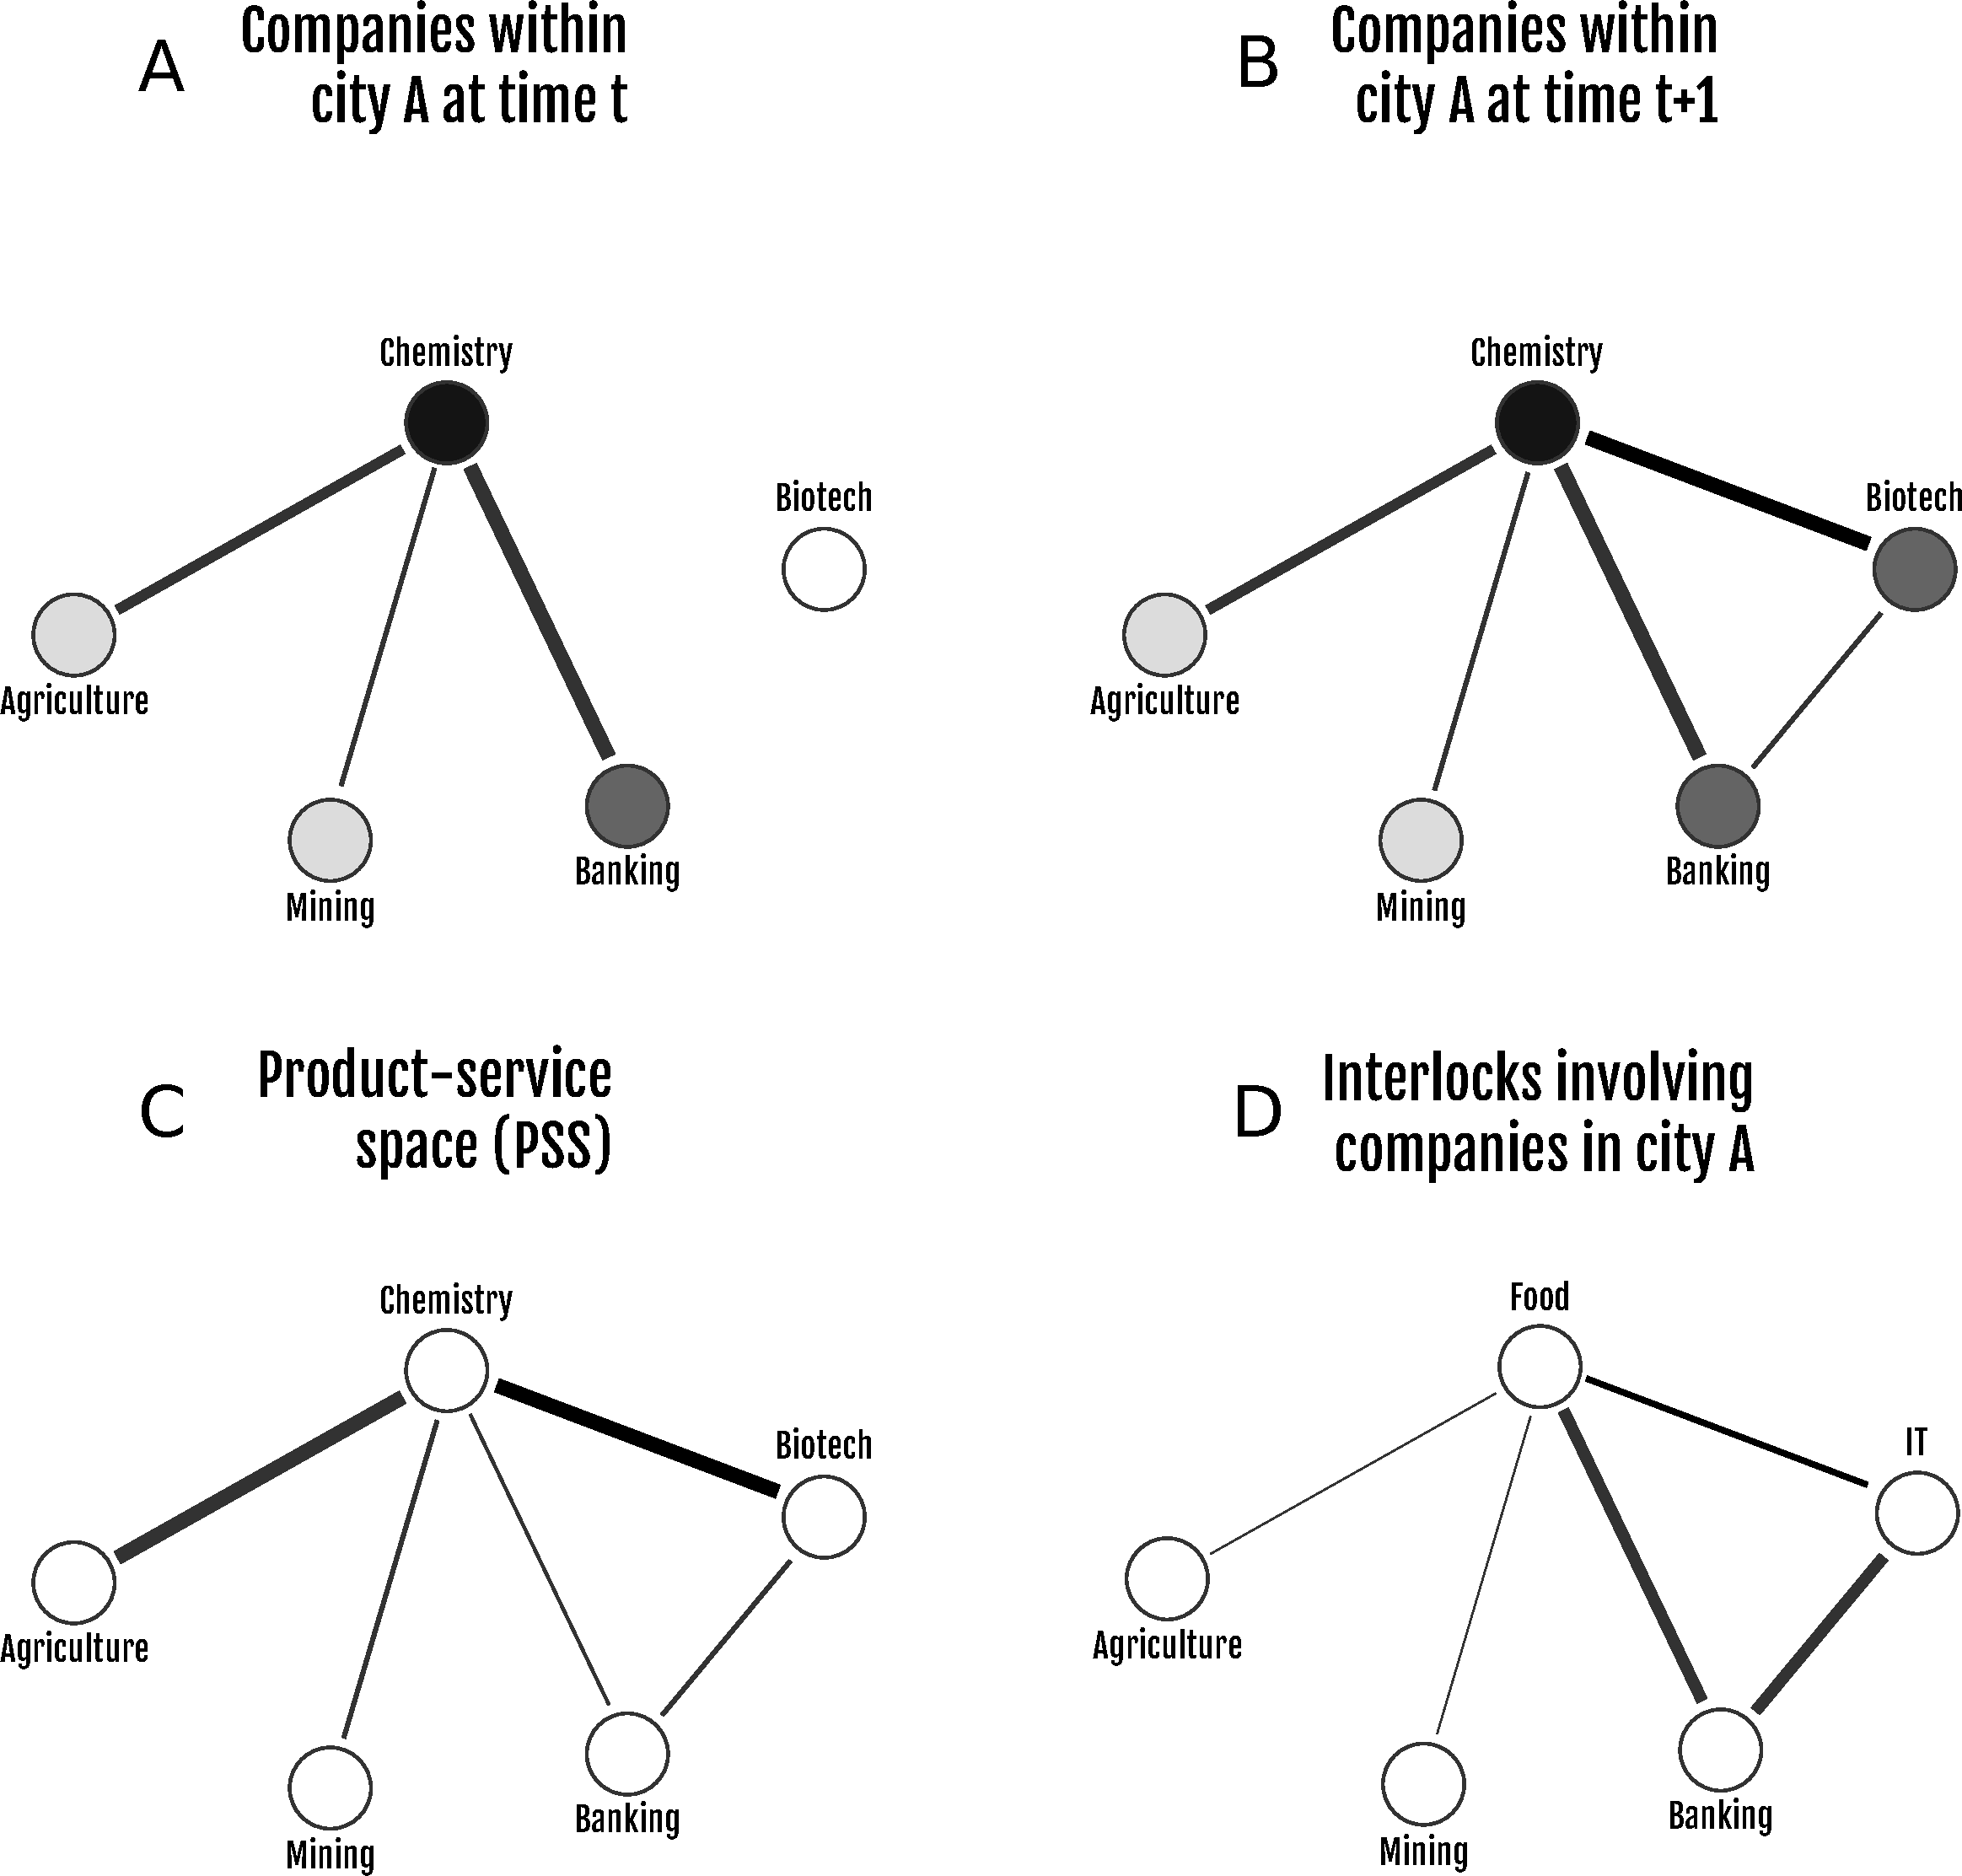
\includegraphics[width=.5\textwidth]{entropy.pdf}
\caption{\textbf{Relation between interlocks, the product-service space, and the distribution of economic activities} (A--B) Distribution of economic activities within a city for times (A) $t$ and (B) $t+1$. The weight of the edges is the product of the number of companies in the nodes (the number of possible opportunities to interlock). (C) The product-space service. The weight of the edges indicate the relatedness of products. (D) Number of interlocks from directors sitting on boards in city A.}
\label{fig:entropy}
\end{center}
\end{figure}

One method to study if interlocks are predictors of the diffusion process is conditional entropy $H(X|Y)$.
The conditional entropy  $H(Companies_{t+1}|Companies_{t})$ quantifies how much extra information we need to define the structure of the network at time $t+1$ knowing the structure at time $t$. 
If the network of interlocks between economic activities affect structural transformation we will find that 
\begin{equation}
\begin{split}
H(Companies_{t+1}|Companies_{t},Interlocks_{t}) \\
< H(Companies_{t+1}|Companies_{t}).
\end{split}
\end{equation}
Other methods include using generative models such as ERGMs~\citep{robins2007introduction} or SIENA~\citep{snijders2008introduction} to assess if the presence of interlocks at time $t$ is predicted by $Companies_{t+1}$,
better than for $Companies_{t}$.
Such a models allow to control for node attributes (see below) and for recursive network effects 
-- e.g. the probability that there is an interlock A--C increases if there are interlocks A--B and B--C (transitivity).

There are several problems with this approach.
Firstly, we have explained that development creates interlocks (endogeneity problem).
The use of longitudinal data allows us to quantify the effect of interlocks on development,
independently of the effect of development on interlocks.
Secondly, there is a chance of self-selection bias.
Companies that want to develop a product in another sector may create interlocks with a company from economic activity beforehand.
However, if this is true, interlocks would also facilitate diffusion.
Finally, a most important bias is omitted variable bias.
If there is an underlying mechanism that produces the interlock at time $t + 1$ and the diffusion at time $t + 2$, 
we would find a false effect of interlocks on the diffusion process.
For example, cities that are developing fast (for whatever reason) may attract more interlocks than those who are not developing.
In order to investigate this possibility, we need to control for city economic indicators, such as infrastructure, resources, education, city size, population density and growth.
Other variables to control are sector size, country indicators and type of interlocks (within city versus between cities).


We can create random models using the product-service space and these variables to investigate their effect.
Importantly, this approach allows us not only to discover if interlocks play a role in the diffusive process, 
but also to unravel what other factors also play a role on it.
Moreover, positive effects of interlocks in the diffusive process would imply that companies should seek interlocks in companies that are adjacent in the product-service space.


\subsubsection{Interlocks affect the product-service space (at least) through innovation}
In section~\ref{sec:interlockspss}, we investigated if interlocks affect the diffusive process in the product-service space.
In this section, we hypothesize that the effect of interlocks in the diffusive process is caused at least partially by an improvement in collaboration and innovation.
Innovation has been linked to gaining competitive advantage~\citep{Hitt1996}, expanding market share ~\citep{Franko1989} and increasing firm performance~\citep{Morbey1988}.
Thus, a correlation in section~\ref{sec:pss} between the product-service space and innovation would not be surprising. 
The subquestion corresponding to this subsection is ``Do interlocks foster collaboration between companies and innovation?''.
We expect interlocks to foster collaboration since directors can assess potential areas of complementarity.
In order to test this hypothesis we will use patent data.
Similarly to the interlock case, two companies are connected if they share a patent.
We can use generative models such as ERGMs or SIENA to assess if the presence of interlocks at time $t$ facilitates the presence of a shared patent at time $t+1$. 
Since we expect other factors to affect the probability of collaboration (such as the presence of a university in the city),
we would need to control for those factors (see ~\ref{sec:interlockspss}).


\subsection{What factors affect interlocks}
\label{sec:factors}
The literature for the factors influencing interlock creation is more consistent.
Geographical distance, colonial history, language, education and social networks have been pointed as factors influencing the presence of interlocks [refs].
Time allowing, we will explore this idea at the micro-scale using generative models such as ERGMs or SIENA.


\subsection{Other projects}
\label{sec:other}
The data allow for the exploration of other projects, such as:
(i) Describe of the inequality among directors, studying if the inequality has its origin in education.
(ii) Analyze the homogenization of coordinated and liberal market economies.
(iii) Quantify the independence of a given sector (e.g. food or media).
(iv) Measure the transference of power from domestic corporation to transnational corporations.
(v) Network motifs, which combination of interlocks between sectors are more likely to occur than random.
(vii) Importance of the nation-state in economic networks.